\documentclass{article}

\usepackage[german]{babel}
\usepackage{array}
\usepackage[letterpaper,top=2cm,bottom=2cm,left=3cm,right=3cm,marginparwidth=1.75cm]{geometry}

\usepackage{amsmath}
\usepackage{graphicx}
\usepackage{subcaption} % Added package
\usepackage[colorlinks=true, allcolors=blue]{hyperref}
\usepackage[T1]{fontenc}
\usepackage{tabularx}
\usepackage{booktabs}


\title{Übungsprotokoll - NWT2 - Übung 03 \\ VLANS}
\author{\vspace{0.5cm} Thomas Brandstätter (s2210239002) \& Jakob Mayr (s2210239021)}

\begin{document}
\maketitle

\section{Konfiguration der Endsysteme}

In der folgenden Übung haben wir die PCs 4.1 und 4.2 benutzt, somit sind die Netze 4.x verwendet worden. Die IP-Konfiguration wird folgendermaßen vergeben: Klick auf „Network“ in der Taskleiste $\rightarrow$ „Network \& Internet Settings“ $\rightarrow$ „Change adapter options“ $\rightarrow$ gewünschtes Netzwerk Interface auswählen, in diesem Fall Ethernet 2 $\rightarrow$ „Properties“ $\rightarrow$ Doppelklick auf „Internet Protocol Version 4“ bzw. „Internet Protocol Version 6“. In den geöffneten Fenstern können wir nun jeweils die IP-Adresse, Subnetzmaske/Präfix und das Gateway eingeben. Folglich sind die Konfigurationen beider PCs zu sehen:

\begin{figure}[!htp]
  \centering
  \begin{minipage}[b]{0.2\textwidth}
    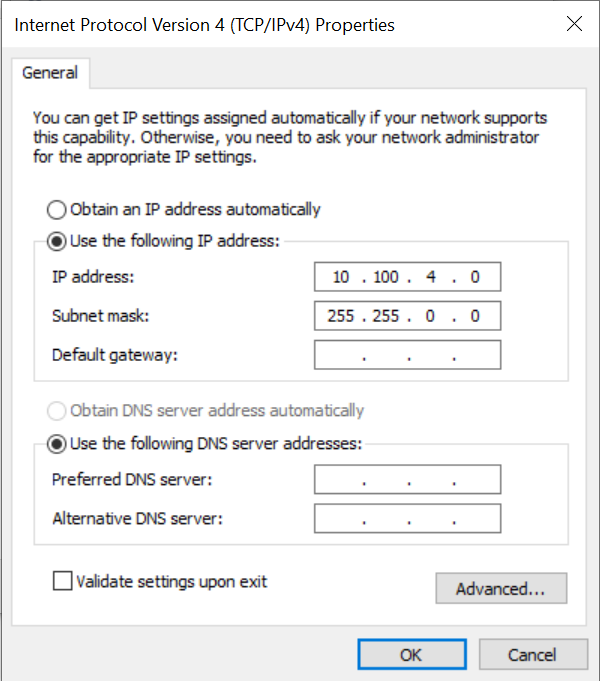
\includegraphics[width=\textwidth]{Arbeitsergebnisse/PC41/pc41_IPv4_config.png}
    \caption{PC41 IPv4 config}
  \end{minipage}
  \hspace{0.8cm}
  \begin{minipage}[b]{0.2\textwidth}
    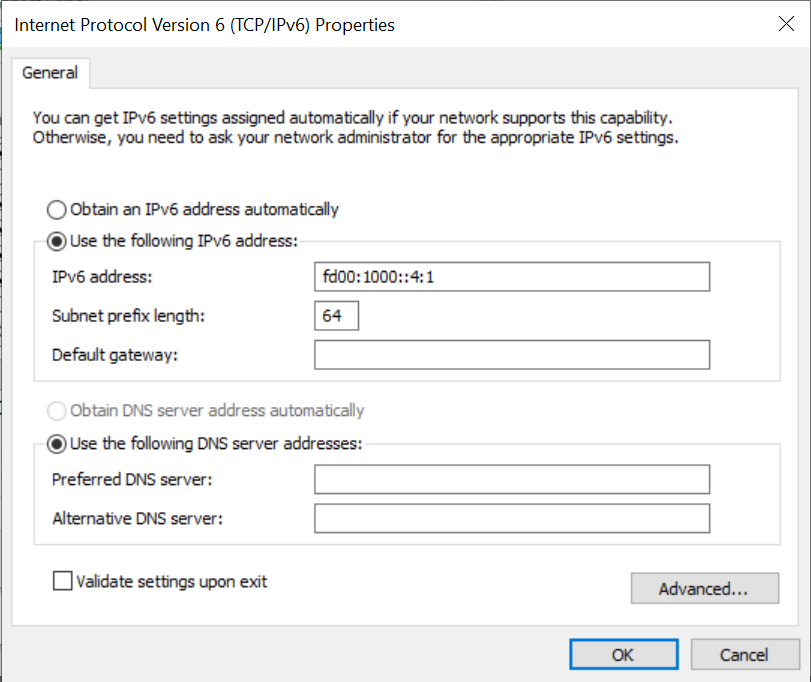
\includegraphics[width=\textwidth]{Arbeitsergebnisse/PC41/pc41_IPv6_config.png}
    \caption{PC41 IPv6 config}
  \end{minipage}
  \hspace{0.8cm}
  \begin{minipage}[b]{0.2\textwidth}
    \includegraphics[width=\textwidth]{Arbeitsergebnisse/PC42/pc42_IPv4_config.png}
    \caption{PC42 IPv4 config}
  \end{minipage}
  \hspace{0.8cm}
  \begin{minipage}[b]{0.2\textwidth}
    \includegraphics[width=\textwidth]{Arbeitsergebnisse/PC42/pc42_IPv6_config.png}
    \caption{PC42 IPv6 config}
  \end{minipage}
\end{figure}

\pagebreak
\section{Konfiguration des Gruppenswitches}

Für die Konfiguration des Gruppenswitches wurden für die Clients die Ports FastEthernet0/11 und FastEthernet0/12, für den Backbone-Switch der Port GigabitEthernet0/1 und für den Gruppenrouter der Port GigabitEthernet0/2 verwendet.
Die Ports für die Clients wurden mit dem "access mode" für die VLANS 41 bzw. 42 konfiguriert.

\begin{table}[htbp]
    \centering
    \begin{tabularx}{\textwidth}{|X|X|}
        \toprule
        \textbf{Befehl} & \textbf{Erklärung} \\
        \midrule
        switchport access vlan <vlan-tag-numbers> & Mit diesem Befehl wird ein Switchport im „access mode“ einem oder mehreren VLANS zugeordnet.\\
        \hline
        switchport mode access & Mit diesem Befehl wird ein switchport in den „access mode“ gesetzt.\\
        \bottomrule
    \end{tabularx}
    \caption{Verwendete Befehle der Switchports für die Clients}
    \label{tab:commands}
\end{table}
\noindent Die Ports für den Backbone-Switch und den Gruppenrouter wurden mit dem „trunk mode“ konfiguriert und haben daher keine zugehörige VLAN-Konfiguration.

\begin{table}[htbp]
    \centering
    \begin{tabularx}{\textwidth}{|X|X|}
        \toprule
        \textbf{Befehl} & \textbf{Erklärung} \\
        \midrule
        switchport mode trunk & Mit diesem Befehl wird ein switchport in den „trunk mode“ gesetzt.\\
        \hline
         switchport trunk allowed vlan <vlan-tag-numbers> & Mit diesem Befehl wird ein switchport im „trunk mode“ einem oder mehreren VLANS zugeordnet.\\
        \bottomrule
    \end{tabularx}
    \caption{Verwendete Befehle der Switchports für Backbone und Router}
\end{table}

\section{Konfiguration des Gruppenrouters}

Für die Konfiguration des Gruppenrouters wurde der Port GigabitEthernet0/0 verwendet. Da das Interface pro VLAN eine unterschiedliche Adressen + Masken benötigt, werden hierfür Subinterfaces (virtuelle Interfaces) verwendet. Das Subinterface GigabitEthernet0/0.42 wird dem VLAN 42 und das Subinterface GigabitEthernet0/0.45 dem VLAN 45 zugewiesen. Zudem muss auf dem Router eine Default-Route zum Backbone-Router konfiguriert werden.

\begin{table}[htbp]
    \centering
    \begin{tabularx}{\textwidth}{|X|X|}
        \toprule
        \textbf{Befehl} & \textbf{Erklärung} \\
        \midrule
        encapsulation dot1Q <vlan-tag-number> & Mit diesem Befehl wird ein Interface einem VLAN zugewiesen.\\
        \hline
        ip address <ip-address> <ip-address-mask> & Mit diesem Befehl wird einem dem ausgewählten Interface eine IPv4-Adresse und Maske zugewiesen.\\
        \hline
        ipv6 address <ip-address/ip-address-mask> & Mit diesem Befehl wird einem dem ausgewählten Interface eine IPv6-Adresse und Maske zugewiesen.\\
        \hline
        ip <routenetwork-number> <network-mask> <ip-address> | interface> & Mit diesem Befehl wird eine statische IPv4 Route in der Routing-Tabelle angelegt.\\
        \hline
        ipv6 <routenetwork-number/network-mask> <ip-address | interface> | interface> & Mit diesem Befehl wird eine statische IPv6 Route in der Routing-Tabelle angelegt.\\
        \bottomrule
    \end{tabularx}
    \caption{Verwendete Befehle für die Konfiguration des Gruppenrouters}
    \label{tab:commands}
\end{table}
\noindent Bei der Konfiguration des Gruppenrouters müssen natürlich wieder das ipv6-unicast-routing (mit dem bereits bekannten Befehl) und der Befehl "no-shutdown" für das Interface verwendet werden.

\section{Fragen zur Konfiguration}

\subsection*{Frage 4.1 \normalfont Warum sind verschiedene VLANs im selben IP Netz nicht sinnvoll}
Da die Eigenschaften von IP-Netzen standardmäßig vorsehen, dass IP-Adressen untereinander "direkt" kommunizieren können ergibt es keinen Sinn ein Netz in VLANs aufzuteilen. Möchte man eine granularere Einteilung kann man das Netz auch in Subnetze trennen.
\subsection*{Frage 4.2 \normalfont Warum müssen auf den Subinterfaces die VLANs bekannt gegeben werden? Warum muss der angeschlossene Switch Port ein Trunk Port sein?}
Standardmäßig würde ein Port im „trunk mode“ alle VLANs routen, da die Aufgabenstellung allerdings verlangt, dass nur bestimmte VLANs geroutet werden können, müssen diese explizit angegeben werden. Ein Trunk Port wird benötigt, damit über diesen Port Netzwerkverkehr von mehreren VLANs geroutet werden können.

\section{Tests und Interpretation ihrer Resultate}

...

\section{Konfiguration}

% \bibliographystyle{alpha}
% \bibliography{sample}

\end{document}

